%# -*- coding: utf-8-unix -*-
%%==================================================
%% chapter02.tex for SJTU Master Thesis
%%==================================================

\chapter{实验分析}
\label{chap:evaluation}

本章节将通过综合性的负载和评测程序来测试SCache对Spark性能的优化效果。
首先我们运行了一个只包含一个shuffle的简单DAG应用来分析硬件利用率的变化。
同时也通过该应用中具体每个任务来分析SCache的优化带来的影响。
之后我们使用了一个公认的含有大量shuffle数据的测试程序Terasort\cite{terasort}来测试不同分区函数下SCache带来的优化。

为了证明SCache能在真实生产环境中带来性能的提升,我们也通过Spark TPC-DS\footnote{https://github.com/databricks/spark-sql-perf}的测试程序来对SCache的优化效果进行测试。

此外我们测试了有权重的水塘采样过程给Spark计算带来的开销。

最后,我们通过模拟的方式对shuffle网络传输过程的进一步优化策略进行测试。


总结来说,SCache的优化可以减少Spark计算过程中89\%的shuffle时间开销。
同时,在单shuffle的DAG程序中,SCache可以帮助Spark实现在reduce阶段75\%的性能提升。
对于Terasort的reduce阶段,在SCache的帮助下可以实现50\%的性能提升。
并且通过启发式预调度算法,相较于Spark调度所产生的经过网络的shuffle数据体积,SCache的优化在加快reduce阶段执行的同时并不会引入额外的网络负载。
在标准的分布式数据库查询评测程序TPC-DS\cite{tpcds}的测试中,经过SCache对shuffle的优化,可以为其中的查询提供接近40\%的平均优化,效果十分显著。

\section{实验平台搭建}

我们在目前应用广泛的Spark分布式计算框架1.6.2版本中实现了SCache的守护进程,并且通过修改Spark核心组件来实现了对DAG中shuffle信息和相关任务信息的提交,SCache附属调度器调度结果的获取和采样程序的插入等,具体可以参考章节\ref{sec:sparkimpl}。
同时,我们租用了亚马逊AWS EC2中50个m4.xlarge类型的节点作为测试平台,并且部署修改后的Spark和SCache。
每个节点的配置如下表所示:
\begin{table}[!hpb]
    \centering
    \bicaption[tab:ec2]{测试平台节点配置}{测试节点平台配置}{Table}{Configuration of Testbed Instance}
    \begin{tabular}{ | m{5cm} | m{8cm} | }
        \hline
        \multicolumn{2}{| c |}{Configuration of Testbed Instance}\\ [0.5ex]
        \hline
        \hline
        Instance Type & m4.xlarge \\ \hline
        CPU & 2.3 GHz Intel Xeon E5-2686 v4 (Broadwell) / 2.4 GHz Intel Xeon E5-2676 v3 (Haswell) \\ \hline
        vCPU & 4 \\ \hline
        Memory & 16GB \\ \hline
        Storage & 8GB SSD, bandwidth 750 Mbps \\ \hline
        Network Bandwidth & N/A, ($\sim$300Mbps as we tested) \\ \hline
        OS & Ubuntu 14.04 LTS \\ \hline
        \hline
    \end{tabular}
\end{table}

其中每个计算节点为一个EC2的虚拟实例,包含了4个vCPU以及16GB的内存和8GB的SSD存储。
以上这些硬件性能保证了在测试过程中CPU和内存不会限制测试程序的计算运行速度,同时也为shuffle数据的缓存提供了较充足的内存空间。
为了给Spark计算提供存储资源,我们还在集群上部署了Hadoop 2.7\cite{hadoop}来提供HDFS的分布式文件系统支持。
除此之外,我们在集群上的每个节点部署了采集CPU磁盘网络等硬件资源利用情况的程序。

\section{单shuffle依赖的DAG执行分析}

我们首先展示了运行与图\ref{fig:util}中一样的,只包含一个shuffle依赖的Spark程序,即Spark GroupByTest\cite{sparksource}。
在此次评测中,我们分别采用了不同体积的输入数据,同时为每一个计算阶段分配了5轮的任务。

在图\ref{fig:scache_util}中展示了在SCache优化下执行该单shuffle依赖的程序时的硬件资源使用情况。
需要注意的是在SCache的优化下,使得整个应用的执行时间缩短了50\%,因此图\ref{fig:scache_util}中横坐标代表的时间长度只有图\ref{fig:util}的一半。
首先可以看到的就是在图\ref{fig:scache_util}中出现了CPU资源利用率峰值和磁盘,网络这些硬件资源利用率峰值的重合。
这表明了通过SCache对shuffle的解耦以及预取,使得节点中硬件资源的利用率和复用率得到了很大的提升。
在更细粒度的硬件资源管理下,SCache避免了在原先Spark中因为I/O的操作而无效的占用计算资源的情况。
同时,由于CPU的资源能被更及时地释放,进而减少了计算资源空置,提高了整个集群在计算过程CPU的利用率。
以上这些硬件资源利用率上的增加和复用率的增加从资源管理效率的角度证明了在SCache的帮助下,Spark的任务能够被更高效的执行,从而获得更好的性能。

\begin{figure}[!htp]
	\centering
	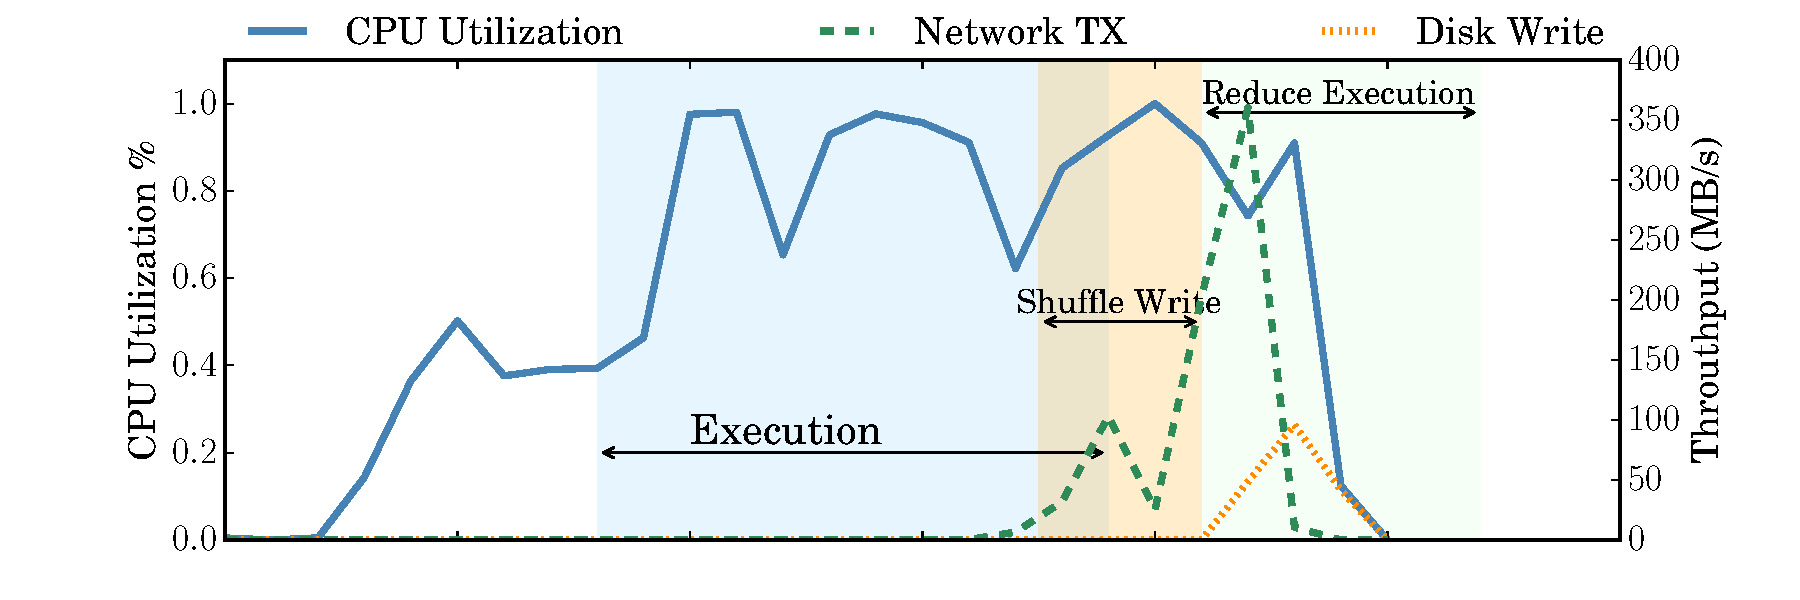
\includegraphics[width=\textwidth]{../../PPoPP-2018/fig/scache_util.pdf}
	\bicaption[fig:scache_util]{SCache优化后运行包含一个shuffle的Spark应用时的硬件资源利用率}{SCache优化后运行包含一个shuffle的Spark应用时的硬件资源利用率}{Fig}{CPU utilization and I/O throughput of a node
	during a Spark Single Shuffle Application with SCache}
\end{figure}

与此同时,我们也在计算任务层面对两者进行了比较。
如图\ref{fig:groupbymapstage}所示,可以看到在map阶段,随着输入数据的体积增加,SCache通过解耦合的方式提前释放CPU资源,同时通过内存拷贝的方式省略磁盘操作。
两者结合,能给map阶段的性能带来一个较为显著的提升。
SCache的优化在map阶段平均可以带来约10\%的性能提升。
而图\ref{fig:groupbyreducestage}展示了shuffle数据预取对于需要大量shuffle数据传输的应用,能在reduce阶段带来显著的性能提升。
这些提升正是因为SCache通过在map阶段对reduce任务实行预调度和shuffle数据的预取,提前了原先Spark模式中shuffle开始的时间,有效地将网络传输时间隐藏在map计算阶段,从而减少了reduce计算阶段启动之后显式的shuffle等待时间,加快了reduce阶段的任务执行。
对于reduce阶段,SCache带来的性能提升较为显著,平均可以达到大约75\%。
两者相结合,在对单shuffle依赖应用的优化过程中,SCache可以减少大约89\%的平均shuffle时间开销。

\begin{figure}[!htp]
	\centering
	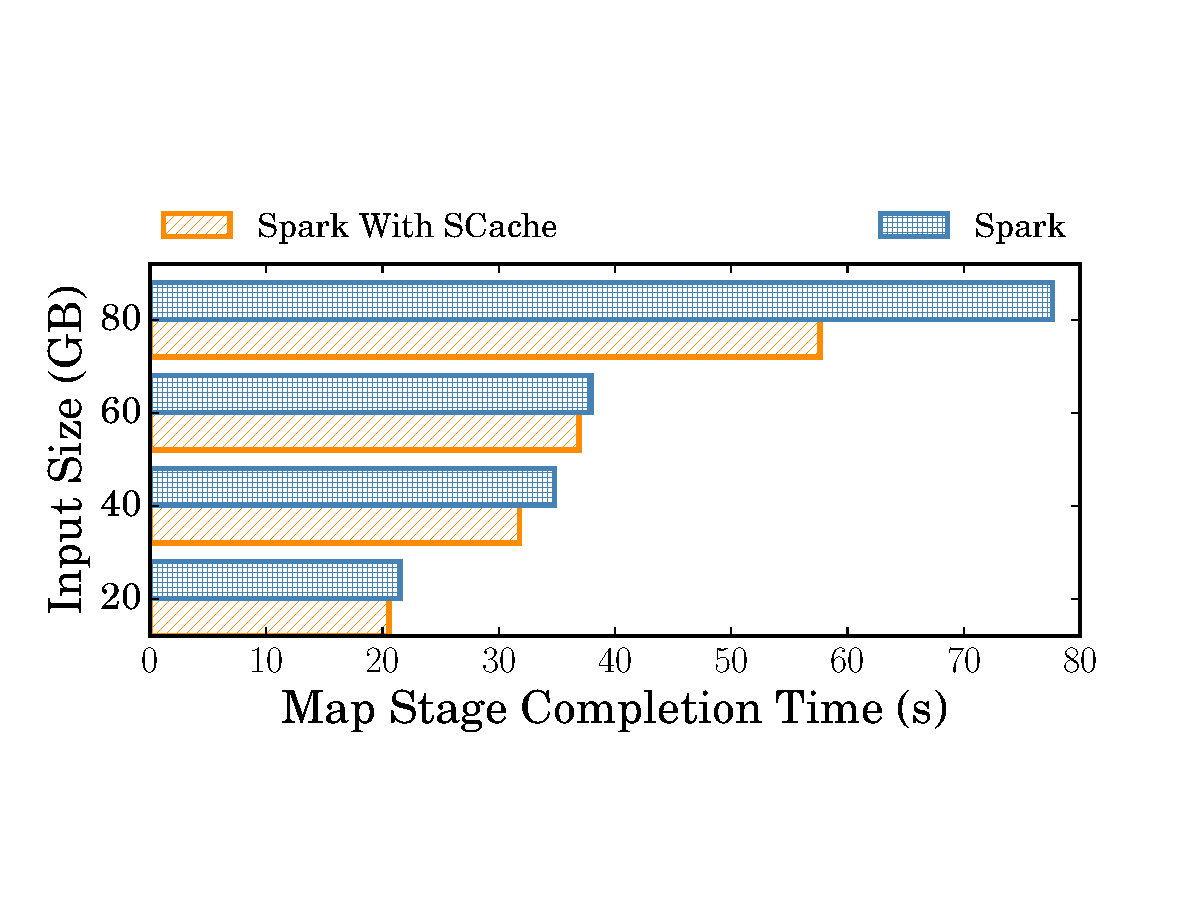
\includegraphics[width=0.7\textwidth]{../../PPoPP-2018/fig/groupbymapstage.pdf}
	\bicaption[fig:groupbymapstage]{单shuffle依赖应用的map阶段完成时间比较}{单shuffle依赖应用的map阶段完成时间比较}{Fig}{Map Stage Completion Time of Single Shuffle Test}
\end{figure}

\begin{figure}[!htp]
	\centering
	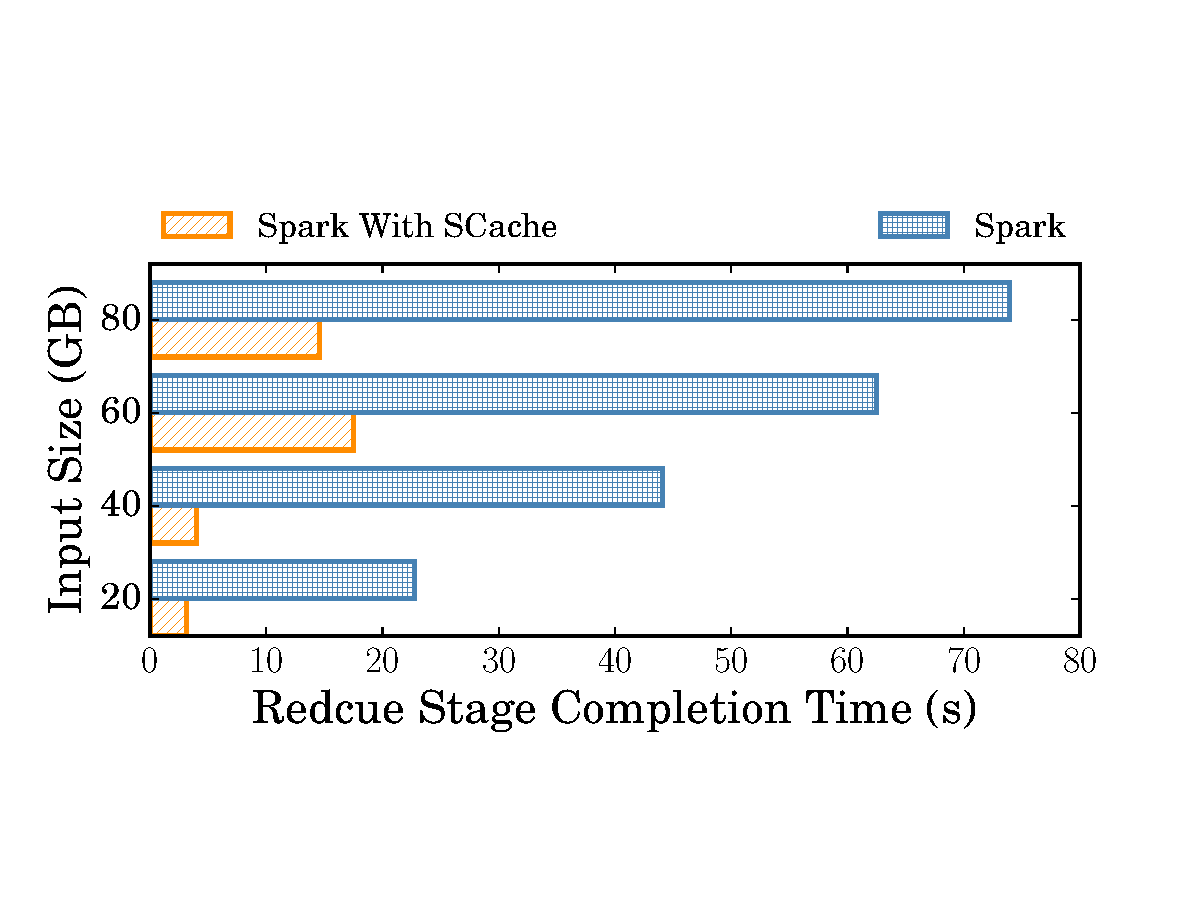
\includegraphics[width=0.7\textwidth]{../../PPoPP-2018/fig/groupbyreducestage.pdf}
	\bicaption[fig:groupbyreducestage]{单shuffle依赖应用的reduce阶段完成时间比较}{单shuffle依赖应用的reduce阶段完成时间比较}{Fig}{Reduce Stage Completion Time of Single Shuffle Test}
\end{figure}

具体到单个计算任务的角度,我们也记录了每个计算阶段中计算任务完成时间处于该阶段所有任务完成时间中位数的那个任务执行过程中具体的时间开销。
如图\ref{fig:groupbymaptask}和图\ref{fig:groupbyreducetask}所示,从任务执行过程中在各个部分的开销,能够进一步验证SCache优化过程的有效性。

在图\ref{fig:groupbymaptask}中的map阶段计算任务的执行过程比较中,可以看到通过SCache的将shuffle的磁盘写操作从map计算任务中解耦合之后,通过内存拷贝的方式可以优化大约40\%的shuffle数据写操作的开销。
之所以SCache的内存拷贝没有完全消除map计算任务中的shuffle写开销是因为在内存拷贝时,首先需要从Spark执行器的Java虚拟机中将shuffle数据移出。
而shuffle数据在Java虚拟机内存内部则是以Java类对象保存的,因此在将其移出内存空间时需要使用序列化的方法将类对象转换成字节码数组。
此处序列化的过程仍然会占用CPU的计算资源和时间\cite{makingsense},并且是不可避免的,因此在图\ref{fig:groupbymaptask}中仍然能观测到shuffle写过程的时间开销。
所以通过对于任务的细粒度分析,也证明了图\ref{fig:groupbymapstage}中,在map阶段SCache解耦shuffle写的过程并没有带来如reduce阶段那么多的提升。

结合图\ref{fig:groupbyreducetask},可以观察到在Spark中,相较于map阶段shuffle写的时间开销,reduce阶段计算任务中shuffle读的开销占到整个任务执行时间的比例更大。
根据我们的实验检测,发现该应用的reduce任务中,shuffle读取过程约占reduce阶段计算任务总时间的50\%。
而这其中的大部分延迟是由网络传输带来的。
SCache通过在map计算阶段的早期对shuffle数据进行了预取,当reduce计算被Spark调度并且开始执行之前,通常情况下只有map计算阶段最后一轮的最后完成的几个任务产生的shuffle数据。
而这部分传输时间由于reduce任务调度的开销以及reduce任务代码序列化等开销,也能被很好的隐藏起来。
因此在第一轮的reduce任务启动之前,SCache根据任务的预调度信息中的reduce任务ID等信息,已经将数据缓存在了内存当中。
在图\ref{fig:groupbyreducetask}中可以看到,SCache可以通过shuffle数据预取将reduce计算任务开始之前的shuffle读等待时间几乎完全的隐藏起来。
也就说在SCache结合上下文的任务预调度与shuffle数据预取机制下,网络传输时间被很好的重叠在了map计算阶段和reduce计算阶段启动时期。

\begin{figure}[!htp]
	\centering
	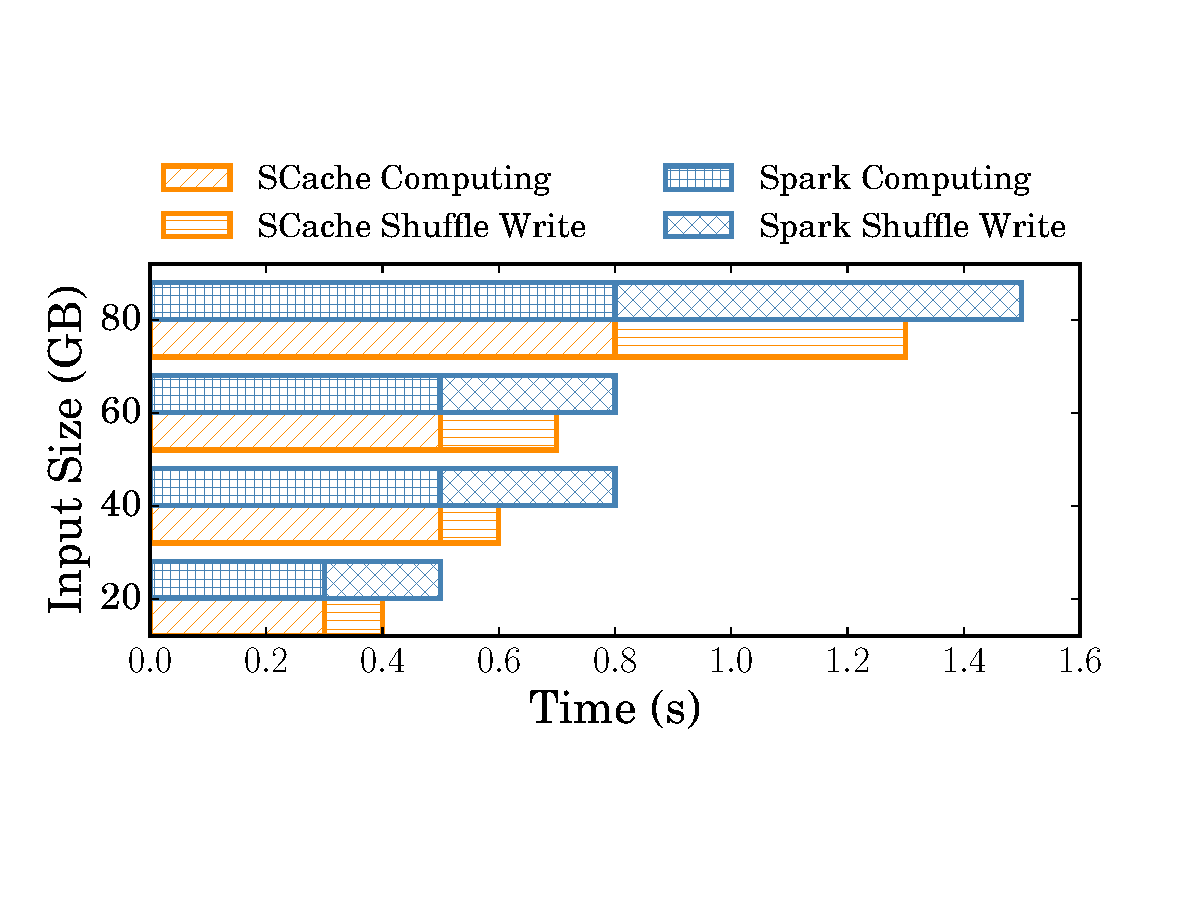
\includegraphics[width=0.7\textwidth]{../../PPoPP-2018/fig/groupbymaptask.pdf}
	\bicaption[fig:groupbymaptask]{单shuffle依赖应用的map阶段中位任务比较}{单shuffle依赖应用的map阶段中位任务比较}{Fig}{Median Map Task Completion Time of Single Shuffle Test}
\end{figure}

\begin{figure}[!htp]
	\centering
	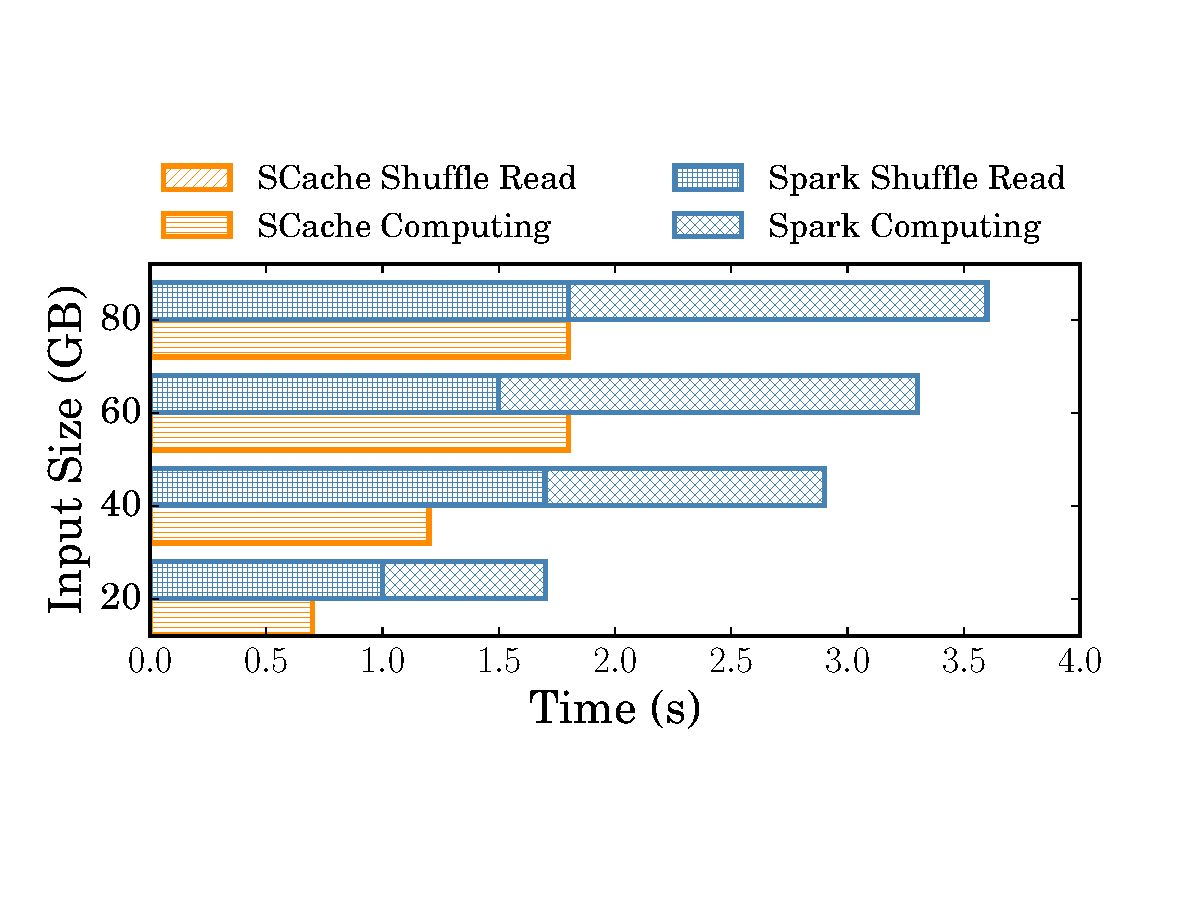
\includegraphics[width=0.7\textwidth]{../../PPoPP-2018/fig/groupbyreducetask.pdf}
	\bicaption[fig:groupbyreducetask]{单shuffle依赖应用的reduce阶段中位任务比较}{单shuffle依赖应用的reduce阶段中位任务比较}{Fig}{Median Reduce Task Completion Time of Single Shuffle Test}
\end{figure}


通过结合map阶段对shuffle数据写的优化以及reduce阶段对shuffle数据读的优化,SCache可以减少Spark的shuffle整体过程大约89\%的shuffle时间开销。

除此之外,在借助启发式算法的reduce任务预调度之后,SCache相较于Spark默认的FIFO算法,在负载均衡上有更好的表现。
在Spark默认的FIFO调度算法下,任务调度器会维护一个调度队列来保存当前仍未被执行的计算任务。
当调度器检测到有计算节点存在计算资源时,就会按照任务ID有小到大依次将任务分配给计算节点。
而默认情况下,一个CPU核心对应了一个slot执行槽,那么这种调度方式很可能会在初始阶段将几个计算量比较大的任务分配到同一个物理节点上,造成该节点的负载过大。
之所以会出现这种情况,是因为Spark默认调度算法并没有把每个任务需要的输入数据体积作为调度的一个参数进行考虑。
而在SCache的启发式算法中,因为调度时通过任务需要的输入体积来估计任务负载,从而将计算量较大的任务均匀分配到了集群的各个节点上,因此相较于Spark默认调度算法能获得更好的负载均衡。
这也是预调度在负载均衡上附带来的一部分优化。

\section{Terasort测试}

Terasort最初作为一个针对MapReduce集群性能测试的测试程序,目前被广泛地用来评测分布式并行计算框架以及其所在集群的性能。
该测试程序主要分为三个部分:数据生成,排序以及验证。
其中的排序部分被广泛的认为是一个需要大量数据进行shuffle的部分。
本文采用了Terasort在Spark上的一个实现\cite{terasort}来测试SCache对于Terasort在排序部分的优化效果。

在数据生成部分,Spark Terasort会根据指定的数据集大小,随机生成相应的测试数据,并存放在分布式存储系统,比如HDFS中。
在数据排序部分,程序首先采用了自定义的哈希分区函数 --- \verb|TeraSortPartitioner|来对数据进行分区。
具体来讲,如代码片段\ref{code:tera}所示,该哈希分区函数结合了用户制定的分区数目(即\verb|numPartitions|),通过对所有随机读入的数据的前缀进行取模计算,从而将该数据划分到对应的reduce计算任务中。
在此过程中,Spark会执行一次shuffle,将数据分别传输到各个reduce任务所对应的分区。
在Terasort的第二阶段,上一步执行的RDD会在此处通过调用\verb|sortByKey()|的方法来在上一步已经粗略分区的基础上进行排序。
在此过程中,Spark首先采用了范围分区函数对现有的RDD进行重新分区,之后就会通过第二次shuffle过程,在reduce阶段对每个分区进行最后的排序。
范围分区函数在这里保证了reduce阶段每个分区都有明确的上下界,从而保证了分区之间的顺序。
而由于在第一阶段使用了根据前缀大小的粗略哈希分区,再加上数据生成部分的随机性,使得这一部分真正需要shuffle的数据量非常小,即shuffle的数据具有很强的本地倾斜性。
根据后续实验,我们发现第二次shuffle的过程中,对于依赖其数据的reduce任务,有93\%的数据是来自于本地某一个map任务的输出。
因此相较于第一个shuffle,在实验中我们将第二个shuffle作为测试SCache预调度机制在极端数据本地倾斜的情况下的调度结果。

\begin{lstlisting}[style={myScalastyle}, caption={Terasort哈希分区函数代码(Scala)}, label={code:tera}]
    val rangePerPart : Long = (max - min) / numPartitions

    def getPartition(key: Any): Int = {
        val b = key.asInstanceOf[Array[Byte]]
        val prefix = Longs.fromBytes(0, b(0), b(1), b(2), b(3), b(4), b(5), b(6))
        (prefix / rangePerPart).toInt
    }
\end{lstlisting}

图\ref{fig:tera}展示对于Terasort中第一个shuffle的测试结果。
这个shuffle是一个典型的有大量网络数据传输的shuffle。
在10GB到200GB的不同体积的输入数据下,经过SCache任务预调度与shuffle数据预取的优化后,Spark的reduce阶段相较于原始的,阻塞式shuffle读取的执行,可以获得将近2倍的加速。
这也符合在单shuffle依赖的执行测试中,SCache在reduce阶段的显著优化效果。

\begin{figure}[!htp]
	\centering
	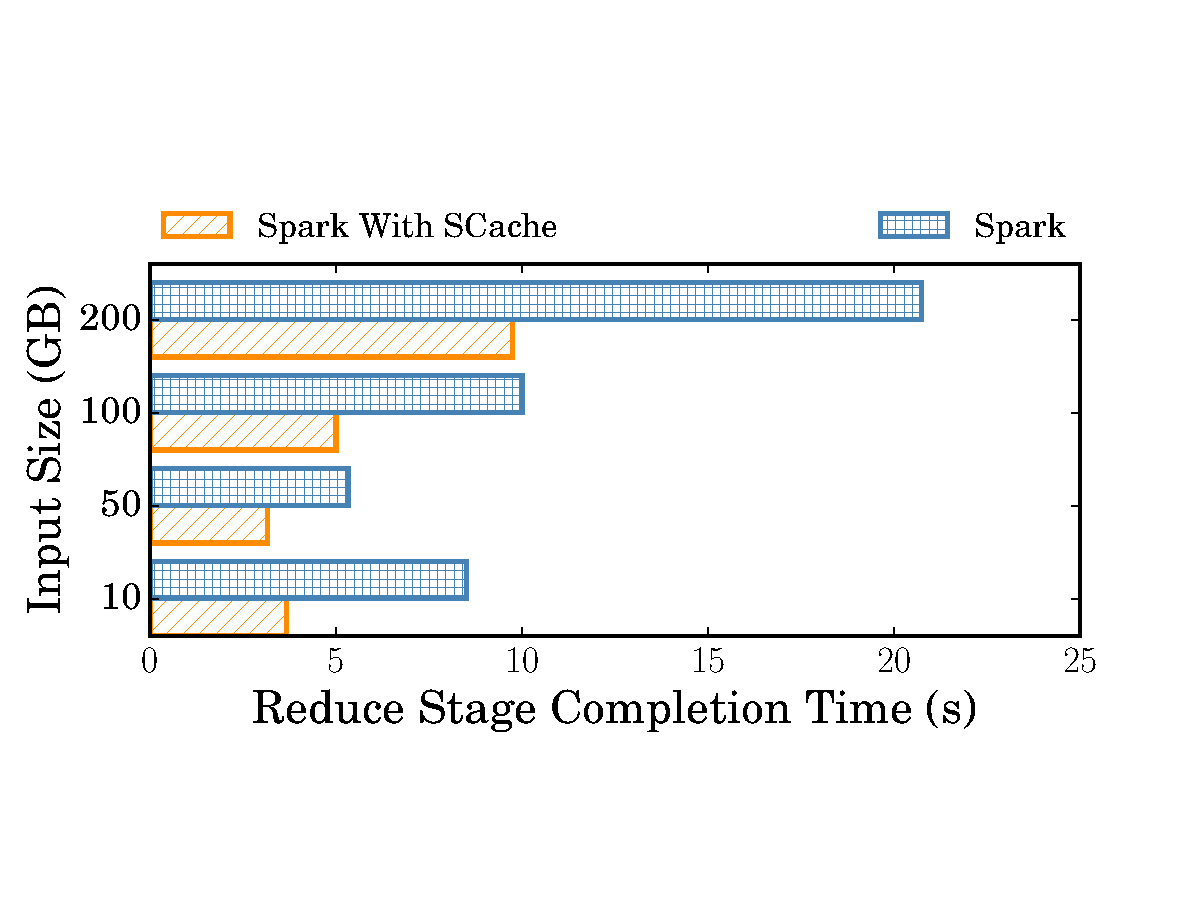
\includegraphics[width=0.7\textwidth]{../../PPoPP-2018/fig/tera.pdf}
	\bicaption[fig:tera]{Terasort第一个shuffle中reduce阶段的完成时间}{Terasort第一个shuffle中reduce阶段的完成时间}{Fig}{Reduce Stage Completion Time of First Shuffle in Terasort}
\end{figure}

图\ref{fig:tera_shuffle}则展示了Terasort的第二个shuffle过程中,SCache与原生Spark分别产生的网络流量。
通过网络的传输数据比较,可以直接反映出在reduce任务调度过程中是否实现了较好的本地性。
如前文所述,该shuffle所产生的数据分布是一个具有极强本地性倾斜的数据。
因此在负载均衡的前提下,最优的调度决策是将某个reduce任务调度到该任务所需输入数据含量最高的一个节点,从而将通过网络的shuffle传输数据降到最低。
Spark在进行该轮调度的时候,通过读取RDD每个数据分区的数据本地性依赖来寻找输入数据含量最高的节点,从而将该数据分区所对应的reduce任务调度到对应的节点上,以获得最小的网络数据传输量。
相对的,SCache则是在map计算阶段通过数据采样的方式来预测shuffle数据的分布,进而预测reduce任务的输入。
在考虑负载均衡的同时,采用启发式的任务置换方式来获取较好的本地性。
在图\ref{fig:tera_shuffle}中可以看出在Terasort的第二个shuffle过程中,SCache的预调度与预取策略产生的网络流量几乎与Spark延迟调度后获得的最优效果一致。
这个实验证明了即使在shuffle数据具有极强的本地性倾斜时,SCache也能通过采样,任务预调度与shuffle预取来获得几乎同样的最优调度结果。

\begin{figure}[!htp]
	\centering
	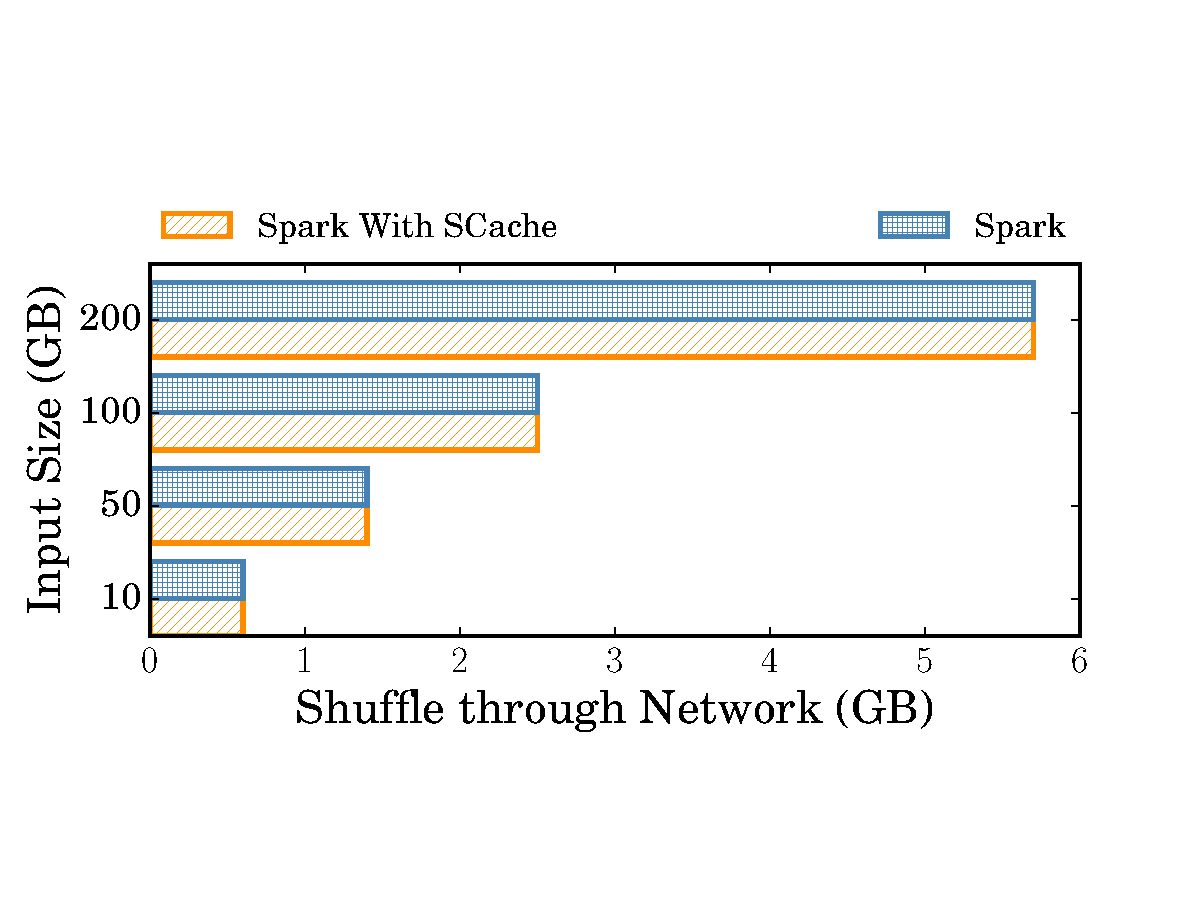
\includegraphics[width=0.7\textwidth]{../../PPoPP-2018/fig/tera_shuffle.pdf}
	\bicaption[fig:tera_shuffle]{Terasort第二个shuffle中网络传输的数据量}{Terasort第二个shuffle中网络传输的数据量}{Fig}{Size of Shuffle Data through Network of Second Shuffle in Terasort}
\end{figure}

\section{生产环境的负载测试}

\begin{figure}[!htp]
	\centering
	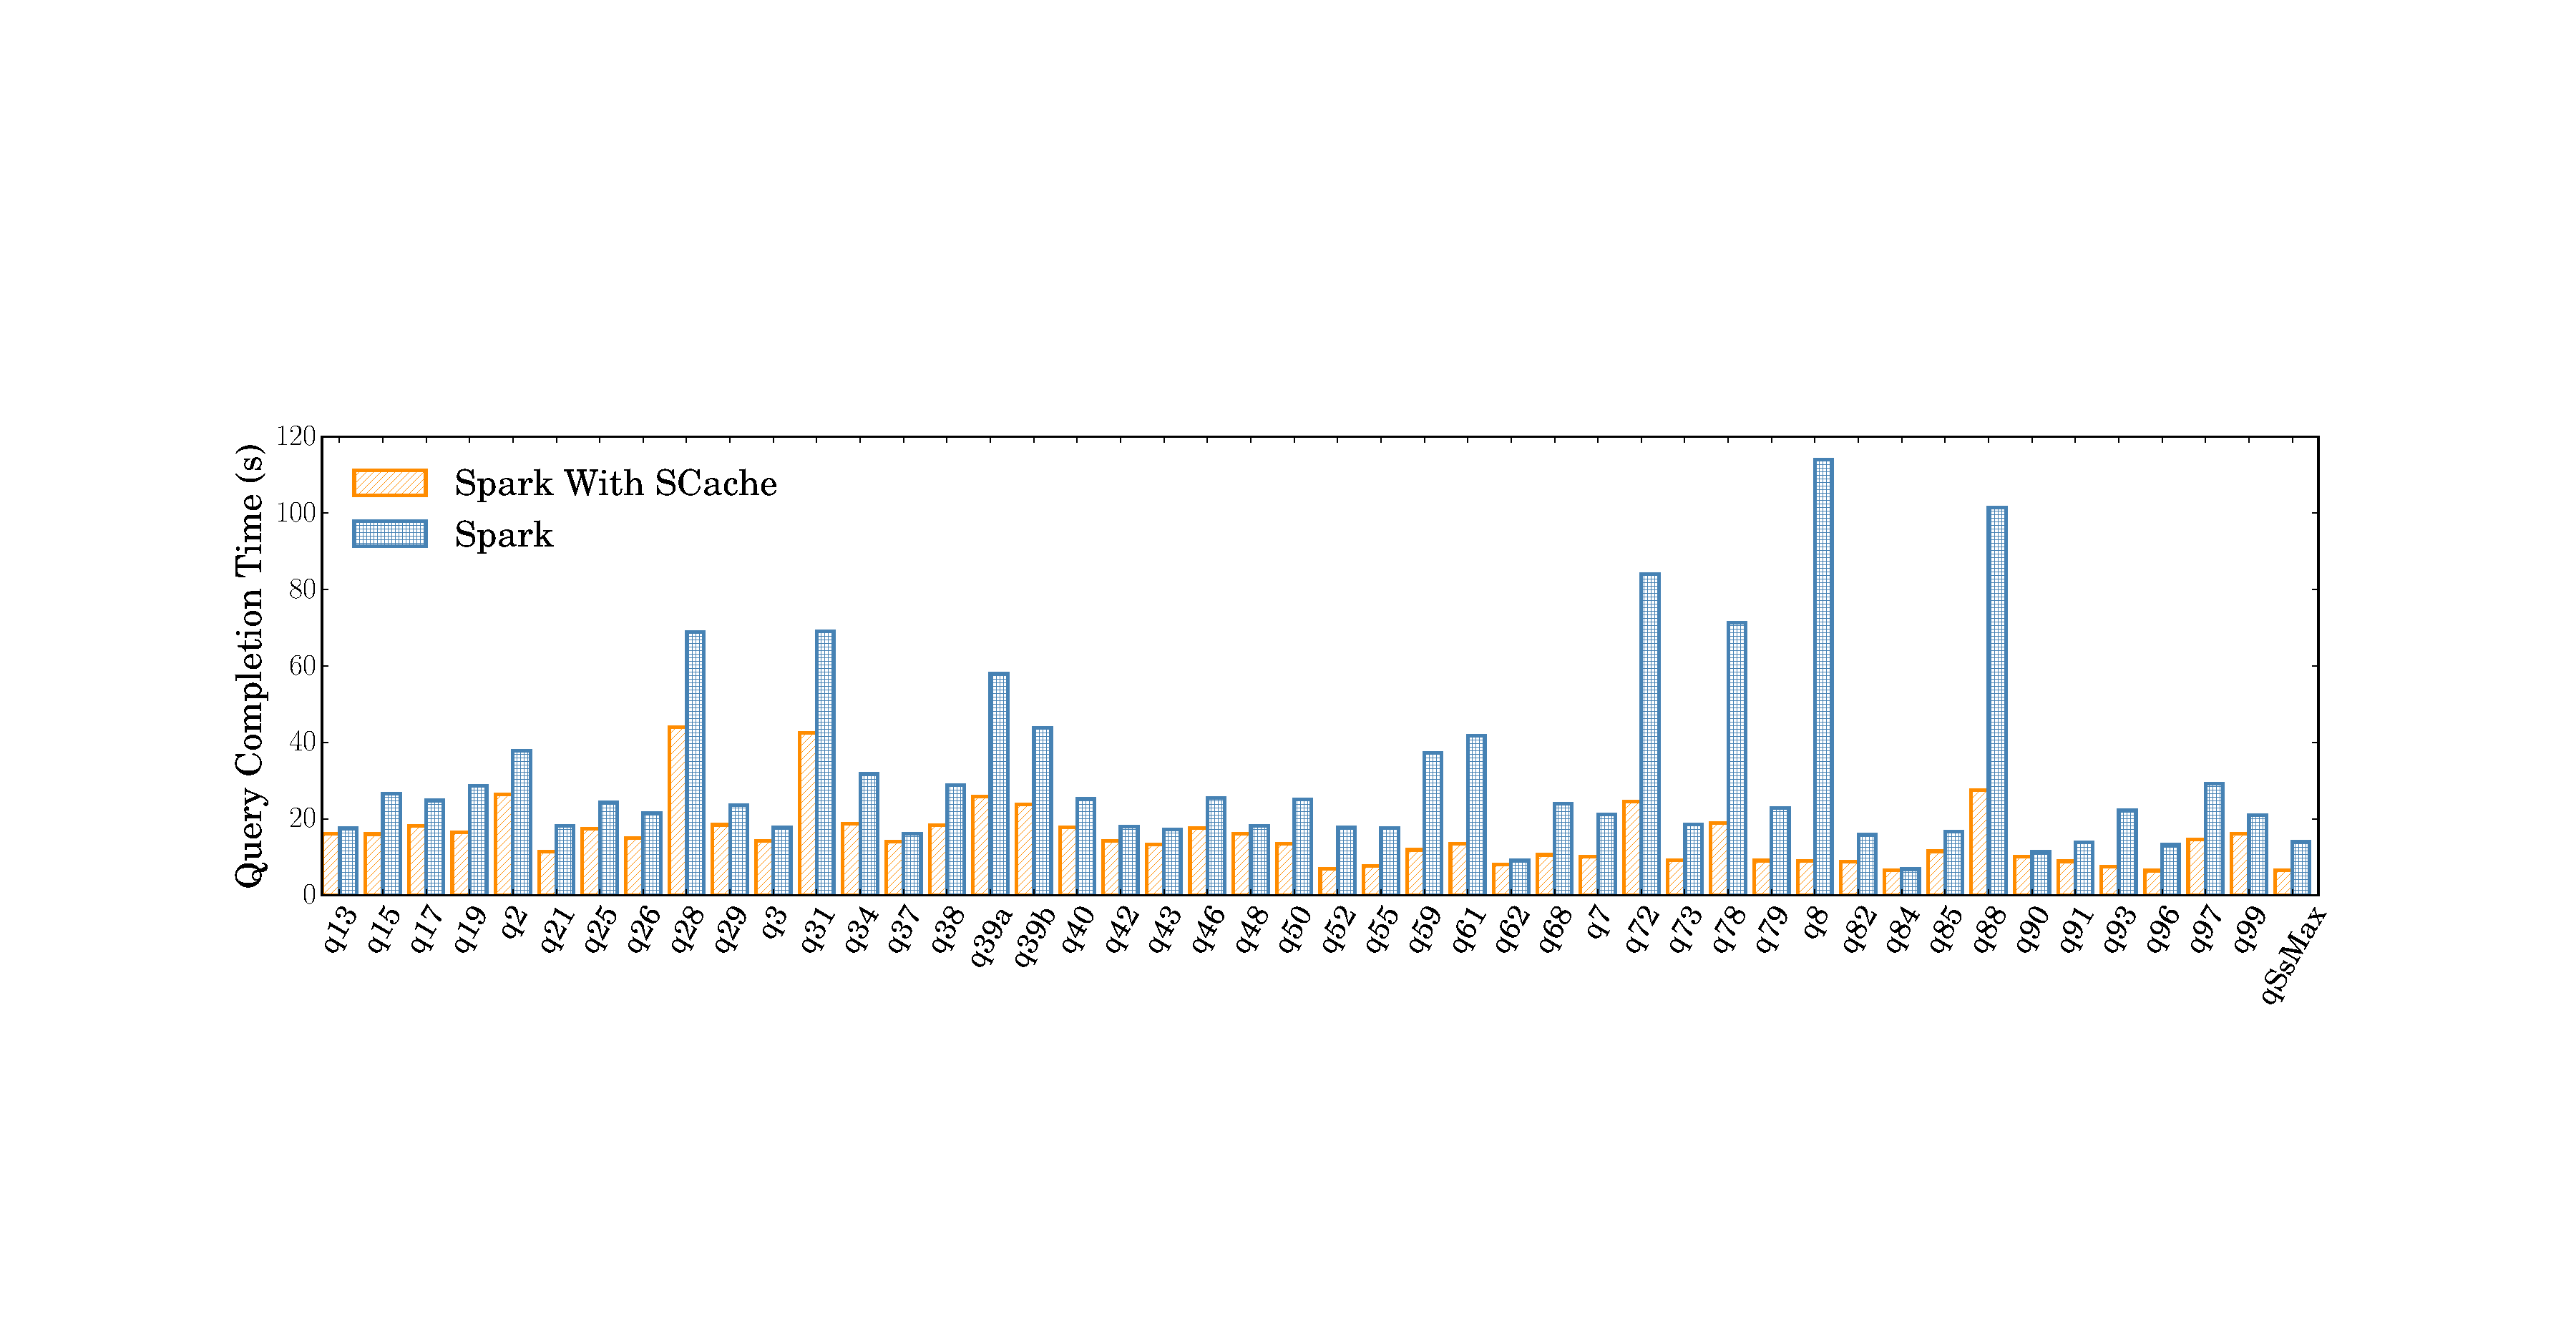
\includegraphics[width=\textwidth]{../../PPoPP-2018/fig/tpcds.pdf}
	\bicaption[fig:tpcds]{TPC-DS测试程序性能比较}{TPC-DS测试程序性能比较}{Fig}{TPC-DS Benchmark Evaluation}
\end{figure}

为了测试SCache对shuffle的优化在真实的生产环境中不同负载情况下的优化性能,我们同样也测试了用于评价分布式数据库检索的标准测试程序TPC-DS\cite{tpcds}。
TPC-DS是一个为数据块查询和数据维持提供通用的模型的测试程序。
它能够在指定的系统环境和配置下,提供对单一用户数据块查询时间的测试,以及多用户模式下,比如ad-hoc,交互式在线分析查询(OLAP),数据挖掘等的查询吞吐的测试。
TPC-DS测试程序是业界用来评测大数据系统性能的标准测试程序之一。
整个TPC-DS测试程序包含了100个不同的数据块查询测试。
由于在Spark 1.6.2上的SQL兼容性问题,使得其中有部分查询不能被正确执行。
所以我们选择了其中一部分可兼容的查询进行测试比较,来观察SCache的shuffle优化效果。
其中有许多查询因为存在多张表的join操作等,会存在较大数据量的shuffle过程。

图\ref{fig:tpcds}展示了原生Spark与在SCache优化下的Spark在执行各个查询的总体时间开销比较。
其中横坐标表示了TPC-DS中的查询测试程序名称,纵坐标则表示每个查询的完成时间。
可以看到由于shuffle在运行中占用了大量的时间开销,使得经过SCache优化后的Spark能获得极大的性能优化。
几乎图中所有的测试,在SCache优化下都能取得显著提升。
更重要的是,在一些查询测试中,比如q8,q72,q88等,在经过SCache对shuffle的优化后,可以获得将近指数级的性能优化。
其根本原因是在这些查询中的大量的“union”,“groupby”等SQL语句在Spark上都会通过shuffle的形式来满足这些数据依赖。
比如图\ref{fig:tpcds}中提升效果最显著的q8,其具体查询代码如代码\ref{code:tpcq8}所示\cite{sparktpcds}:

\begin{lstlisting}[language={SQL}, caption={TCP-DS的q8查询代码片段}, label={code:tpcq8}]
    select s_store_name, sum(ss_net_profit)
    from store_sales, date_dim, store,
        (SELECT ca_zip
          from (
          (SELECT substr(ca_zip,1,5) ca_zip FROM customer_address
             WHERE substr(ca_zip,1,5) IN (
                  '24128','76232','65084','87816','83926','77556','20548',
                  '26231','43848','15126','91137','61265','98294','25782',
                  '...',    -- numbers of integer are omitted
                  '17871','35258','31387','35458',
                  '35576'))
          INTERSECT
          (select ca_zip
             FROM
               (SELECT substr(ca_zip,1,5) ca_zip,count(*) cnt
                 FROM customer_address, customer
                 WHERE ca_address_sk = c_current_addr_sk and
                       c_preferred_cust_flag='Y'
                 group by ca_zip
                 having count(*) > 10) A1)
            ) A2
         ) V1
    where ss_store_sk = s_store_sk
     and ss_sold_date_sk = d_date_sk
     and d_qoy = 2 and d_year = 1998
     and (substr(s_zip,1,2) = substr(V1.ca_zip,1,2))
    group by s_store_name
    order by s_store_name LIMIT 100
\end{lstlisting}

可以看到在TPC-DS的q8查询中存在对大量数据的\verb|INTERSECT|,\verb|groupby|,\verb|orderby|等操作,这些操作的背后都会存在大量的shuffle,因此在这个测试中,SCache通过对shuffle的优化使Spark在端到端的工作完成时间上获得了巨大的提升。

平均各个查询的完成时间,经过SCache的优化可以使TPC-DS这些查询获得平均40\%的完成时间上的提升。
在TPC-DS上的实验证明即使对于在真实生产环境中的端到端的任务完成时间,SCache对于shuffle的优化仍然是非常有前景的。

\section{采样的开销}

在这一章节,我们测试了采样过程在整个shuffle优化中的开销。
对于采样过程的开销,我们主要从两个维度对其进行测量 --- 集群中节点数量和每个节点输入数据的体积。
其中为了保证系统的可扩展性,采样的开销相对于集群体积的变化规律更为重要。
因为如果采样的开销会随着集群中节点数量增加而增加的话,即使这种关系是线性的,那么也将极大的影响到SCache的可扩展性。
虽然系统在设计时采用了主从节点的传统集中式控制模式,但是由于中心节点的负载相对较低,且其所管理的shuffle相关元数据量仅局限于一个DAG应用的运行时间范围,甚至是一个shuffle的时间内,因此其中心节点的负载很难成为整个集群扩展的瓶颈。
综上所述,采样的开销是否会限制SCache的可扩展性将成文本次测试的重点。

\begin{figure}[!htp]
	\centering
	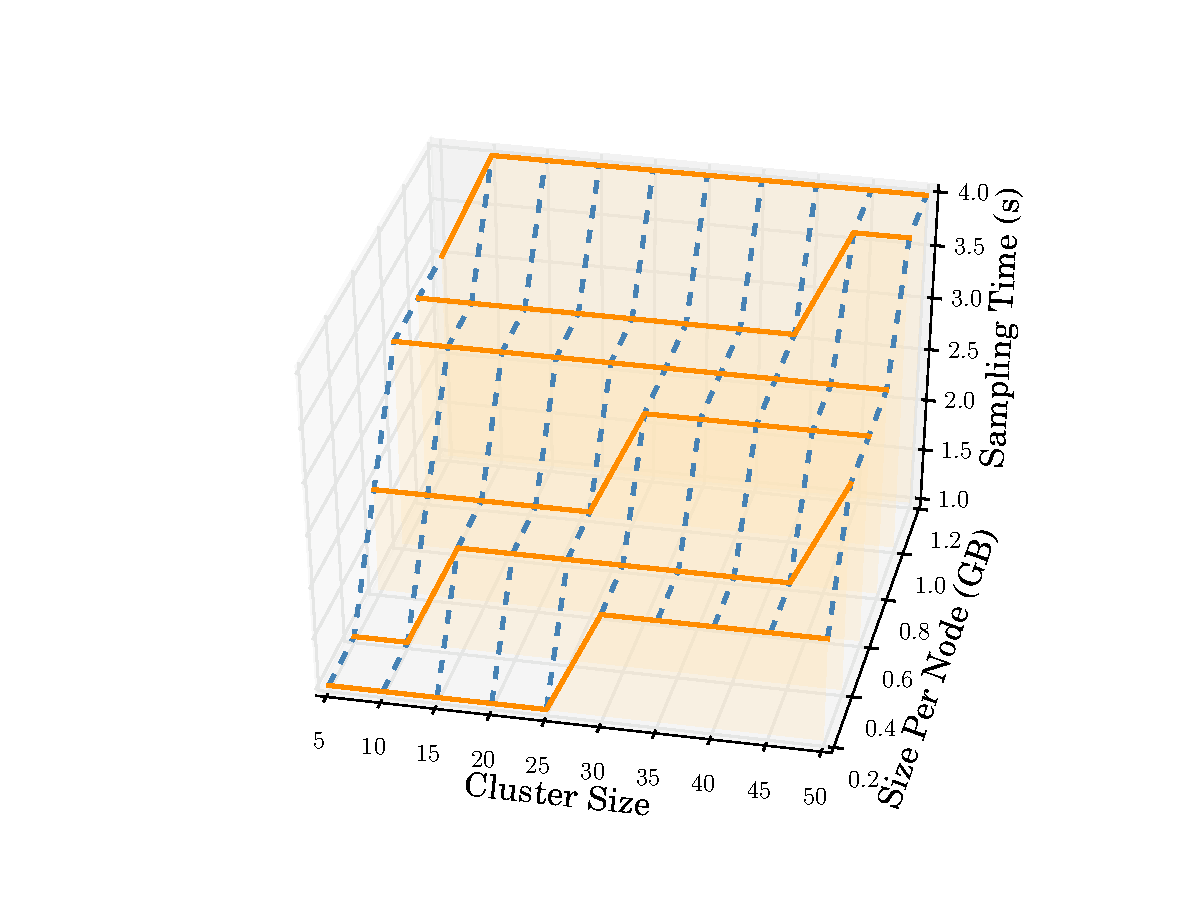
\includegraphics[width=0.6\textwidth]{../../PPoPP-2018/fig/sampling.pdf}
	\bicaption[fig:sampling]{采样过程的开销}{采样过程的开销}{Fig}{Sampling Overhead}
\end{figure}

图\ref{fig:sampling}展示了在两个维度下SCache采样过程的开销。
在相同集群节点数目下,随着每个节点输入数据体积的增加,采样的开销相应的也有所增加(图\ref{fig:sampling}中的点状线)。
可以看到采样开销与每个节点输入数据量基本成线性关系,这个和采用水塘采样算法进行抽样的算法设计相符,在目前的设计中无法避免。
因为虽然采样程序(等式\ref{eq:sample})只对固定样本数的数据进行计算和分区,但是仍然需要统计输入数据中键值对的数量。
因此随着数据体积增加,开销接近线性的增长也与设计相吻合。
所幸是采样开销的绝对值相对较低,并不会给整个DAG应用的执行带来很大影响。

而图\ref{fig:sampling}中实线线条所展示的则是在相同的每个节点输入数据体积下,随着集群中节点数量的增加,采样开销的变化。
可以看到除了在每个节点输入数据体积为0.4GB的情况下,采样开销随着集群中节点数增加有两次的上升以外,在其他体积下,采样数并没有随着集群节点数的增加而上升。
基本上可以断定采样的开销在集群中节点数目的变化的维度是相对稳定的。
此处采样开销的稳定主要得益于中心节点对于每个节点采样数据的收集相对简单。
首先中心节点收集单节点的数据量是固定的,只包含了采样后的输出数据分布和对应的输入数据体积值,这些数据并不受节点的输入数据体积影响。
与此同时,由于单节点所需上传的数据较少,因此对于网络传输也不会带来过高的负载。
而对于中心节点在基于上述收集数据后的计算,我们也考虑到预测算法与预调度算法的复杂性,尽可能的用时间复杂度较低的算法来完成预测和任务预调度。
综上所述,采样过程的开销在集群节点数的维度上能保持相对稳定,而实验结果也很好的证明了在设计过程中的优化措施,使得中心节点不会成为影响整个集群可扩展性的瓶颈。

\section{网络层优化}

在本章节我们对shuffle网络传输通过coflow的调度系统的进一步优化做了评测。
受限于Amazon EC2虚拟机集群对网络的不可控,在实现过程中不能将coflow的调度优化系统集成到SCache之中。
因此本次测试将通过模拟实验的方式呈现。

在测试过程中,我们使用了在章节\ref{chap:optimization}中提到的OpenCloud公开的日志文件中的shuffle数据。
其体积分布如图\ref{fig:cdf}所示。
由于SCache能够提供coflow调度所需的所有信息,因此我们在这里采用了Varys\cite{varys}和Seagull\cite{seagull}中在信息已知下相对最高效的调度算法 ---
Smallest-Effective-Bottleneck-First(SEBF)和Minimum-Allocation-for-Desired-Duration(MADD)的结合。
当有多个shuffle网络传输所组成的coflow准备开始传输时,在SEBF的算法调度下,coflow调度系统会根据其中coflow的长度(即$length$),将长度最小的coflow赋予最高的优先级,最早进行传输。
而在MADD的算法策略下,coflow调度系统会将其中所有的网络流的完成时间拖慢到与每个coflow的长度一样,从而可以让出更多的带宽给其他网络流传输。

\begin{figure}[!htp]
	\centering
	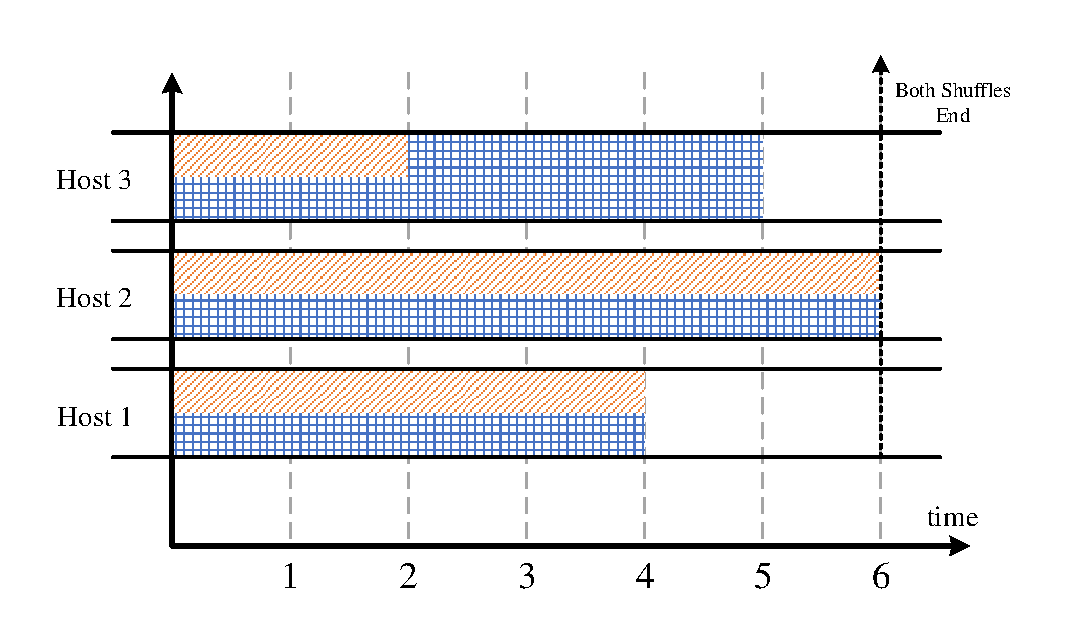
\includegraphics[width=0.8\textwidth]{coflowfair.pdf}
	\bicaption[fig:coflowfair]{传统网络的平均调度策略}{传统网络的平均调度策略}{Fig}{Per-flow Fairness Network Scheduling}
\end{figure}

举例来说,图\ref{fig:coflowfair}所示,有两个shuffle所对应的coflow同时开始网络传输,其中每个coflow分别包含三个网络流。
橙色斜线coflow(coflow 1)的三个网络流从节点Host 1至Host 3的体积分别是2,3,1。
蓝色十字coflow(coflow 2)的三个网络流从节点Host 1至Host 3的体积分别是2,3,4。
在传统的网络调度下,系统会最终使两个网络流平均共享一个链路。
因此对于coflow 1和coflow 2在平均调度策略的调度下,两者的完成时间均是6。
所以其平均coflow完成时间
\begin{equation}
    average\, CCT = \frac{6 + 6}{2} = 6。
\end{equation}
而在SEBF的策略中,如图\ref{fig:coflowsebf}所示,coflow 1的长度为3,而coflow 2的长度为4,因此coflow 1将优先传输。
与此同时,MADD算法会将coflow 1中其他两个体积较小流的完成时间延长到与其长度3一致。
因此让出来的部分带宽资源,供coflow 2传输使用。
在这种调度策略下,coflow 1的完成时间是3,而coflow 2的完成时间是6。
所以其平均coflow完成时间
\begin{equation}
    average\, CCT = \frac{3 + 6}{2} = 4.5。
\end{equation}

\begin{figure}[!htp]
	\centering
	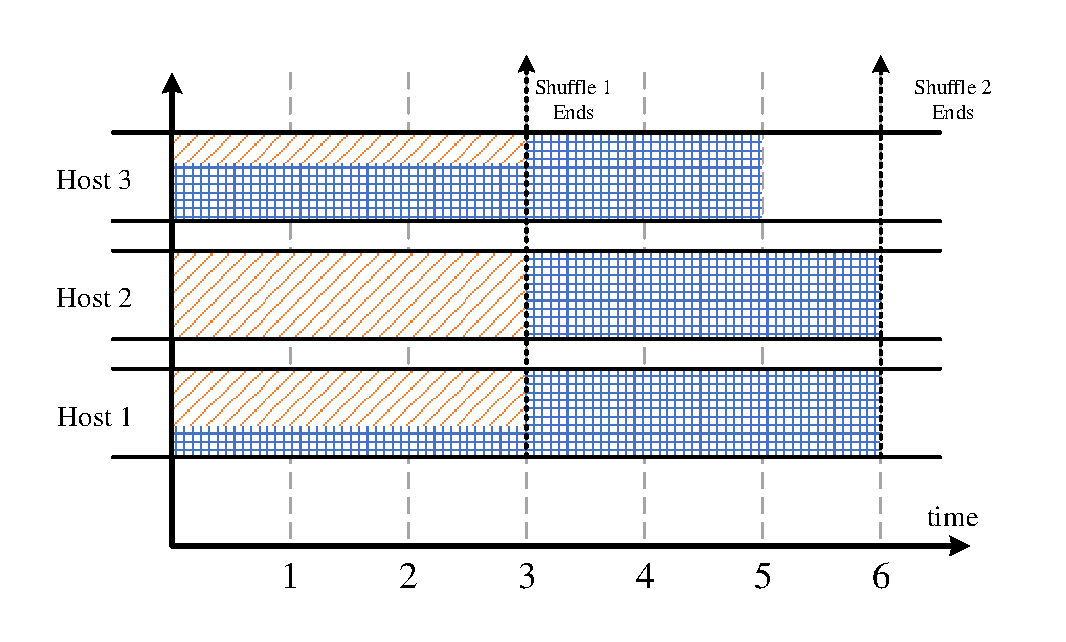
\includegraphics[width=0.8\textwidth]{coflowsebf.pdf}
	\bicaption[fig:coflowsebf]{SEBF和MADD的网络调度策略}{SEBF和MADD的网络调度策略}{Fig}{SEBF with MADD Network Scheduling}
\end{figure}

除了应用这两个算法对shuffle对应的coflow的优先级进行优先级调度和速度限制之外,我们还考虑了链路带宽的不稳定对限速精确性带来的影响。
因为集群中的带宽不仅仅专属于分布式DAG计算框架,往往分布式存储系统,资源调度系统等都会利用集群中的网络来传输数据和信号信息,所以在模拟过程中,我们通过Seagull\cite{seagull}中提到的带宽检测方案,
将网络链路剩余带宽的体积也考虑到调度中来。

\begin{figure}[!htp]
	\centering
	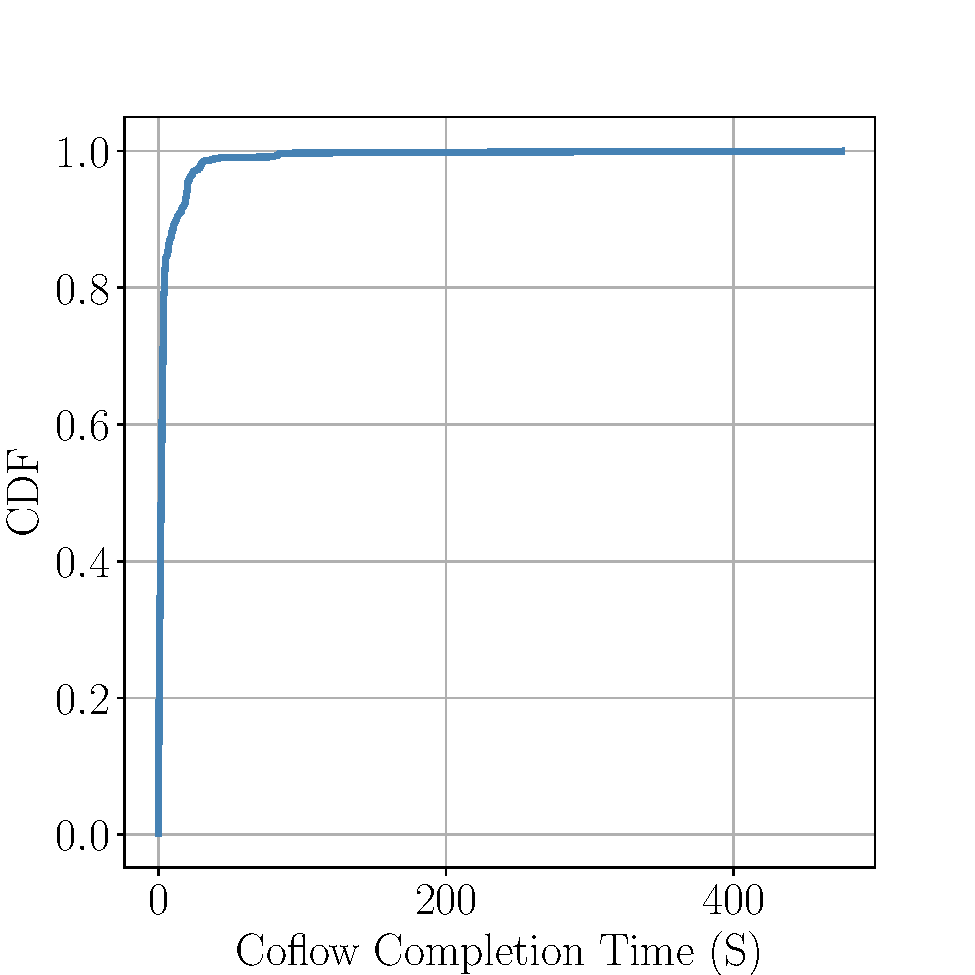
\includegraphics[width=0.6\textwidth]{coflow_cdf.pdf}
	\bicaption[fig:coflowcdf]{OpenCloud日志中Coflow完成时间累积分布}{OpenCloud日志中Coflow完成时间累积分布}{Fig}{Coflow Completion Time CDF of OpenCloud Trace}
\end{figure}

\begin{figure}[!htp]
	\centering
	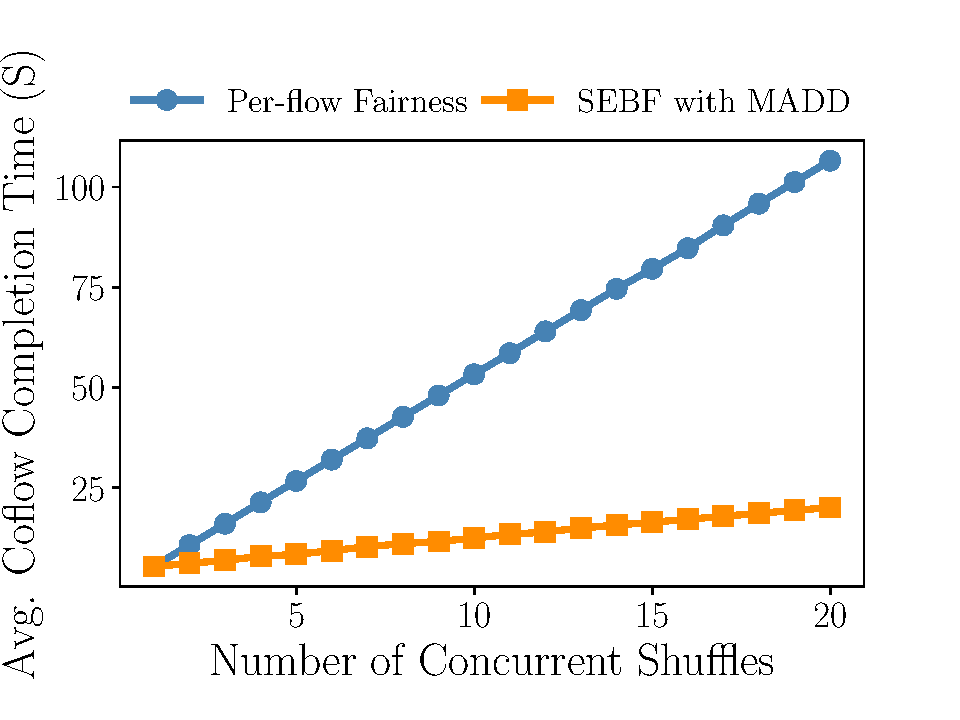
\includegraphics[width=0.7\textwidth]{coflowsim.pdf}
	\bicaption[fig:coflowsim]{不同调度策略下的shuffle网络传输模拟实验}{不同调度策略下的shuffle网络传输模拟实验}{Fig}{Simulation of Shuffle Network Transfer under Different Scheduling Schemes}
\end{figure}

在模拟实验中,我们抽取了OpenCloud中所有任务的shuffle数据,并且通过对每个应用对应的shuffle时间进行聚合,形成一个coflow调度单元。
对于每一个coflow单元,他们独自占用模拟实验中的网络时的完成时间累积分布如图\ref{fig:coflowcdf}所示。
其平均完成时间5.33秒,从图\ref{fig:coflowcdf}中可以看出其中大部分该日志中的shuffle网络传输时间均集中在平均值附近,只存在少量大体积的shuffle传输。
这也与图\ref{fig:cdf}中得出的结论匹配,即OpenCloud日志中大部分应用的shuffle开销较小。

根据这些coflow单元的数据,实验随机模拟了不同等级并发量的shuffle同时传输的情景,通过传统网络的平均调度策略,以及SEBF和MADD算法分别对当下并发的shuffle传输进行调度。
模拟实验在不同算法以及并发量下求出了每个并发shuffle下的coflow平均完成时间(average CCT)。
实验结果如图\ref{fig:coflowsim}所示。

可以看到随着shuffle并发量的增加,传统网络调度策略对shuffle的网络传输过程就越不利。
结合图\ref{fig:coflowcdf}可以看到,由于OpenCloud的日志里面的shuffle的体积分布都集中在平均值附近,所以随着并发量的增加,在传统调度策略下,shuffle的完成时间也随之呈线性的增加。
而经过SEBF和MADD算法的优化调度之后,shuffle完成时间随着并发量增加的幅度相对较小。
当并发量达到20时,两者的性能差距甚至能达到将近10倍。
通过上述实验可以看出在网络层面通过coflow的调度进一步对shuffle的网络传输部分进行优化能够给整个shuffle优化过程带来更大的性能提升。
